\title{Unsupervised learning}

\subsection{Unsupervised learning}

In unsupervised learning, the task is to infer hidden structure from
unlabeled data, comprised of training examples $\{x_n\}$.

We demonstrate how to do this in Edward with an example.
The script is available at
\href{https://github.com/blei-lab/edward/blob/master/examples/mixture_gaussian_collapsed.py}
{\texttt{examples/mixture_gaussian_collapsed.py}} in the Github repository.

\subsubsection{Data}

Use a simulated dataset of 2-dimensional datapoints
$\mathbf{x}_n\in\mathbb{R}^2$.
\begin{lstlisting}[language=Python]
def build_toy_dataset(N):
  pi = np.array([0.4, 0.6])
  mus = [[1, 1], [-1, -1]]
  stds = [[0.1, 0.1], [0.1, 0.1]]
  x = np.zeros((N, 2), dtype=np.float32)
  for n in range(N):
    k = np.argmax(np.random.multinomial(1, pi))
    x[n, :] = np.random.multivariate_normal(mus[k], np.diag(stds[k]))

  return x

N = 500  # number of data points
D = 2  # dimensionality of data

x_train = build_toy_dataset(N)
\end{lstlisting}

We visualize the generated data points.
\begin{lstlisting}[language=Python]
plt.scatter(x_train[:, 0], x_train[:, 1])
plt.axis([-3, 3, -3, 3])
plt.show()
\end{lstlisting}
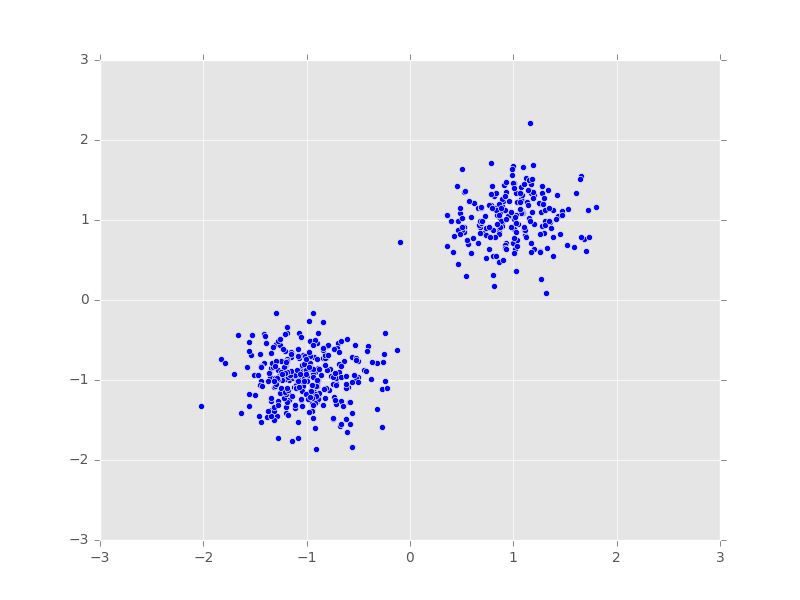
\includegraphics[width=700px]{/images/unsupervised-fig0.png}

\subsubsection{Model}

A mixture model is a model typically used for clustering.
It assigns a mixture component to each data point, and this mixture component
determines the distribution that the data point is generated from. A
mixture of Gaussians uses Gaussian distributions to generate this data
\citep{bishop2006pattern}.

For a set of $N$ data points,
the likelihood of each observation $\mathbf{x}_n$ is
\begin{align*}
  p(\mathbf{x}_n \mid \pi, \mu, \sigma)
  &=
  \sum_{k=1}^K \pi_k \, \text{Normal}(\mathbf{x}_n \mid \mu_k, \sigma_k).
\end{align*}
The latent variable $\pi$ is a $K$-dimensional probability vector
which mixes individual Gaussian distributions, each
characterized by a mean $\mu_k$ and standard deviation $\sigma_k$.

Define the prior on $\pi\in[0,1]$ such that $\sum_{k=1}^K\pi_k=1$ to be
\begin{align*}
  p(\pi)
  &=
  \text{Dirichlet}(\pi \mid \alpha \mathbf{1}_{K}).
\end{align*}

Define the prior on each component $\mathbf{\mu}_k\in\mathbb{R}^D$ to be
\begin{align*}
  p(\mathbf{\mu}_k)
  &=
  \text{Normal}(\mathbf{\mu}_k \mid \mathbf{0}, \sigma^2\mathbf{I}).
\end{align*}

Define the prior on each component $\mathbf{\sigma}_k\in\mathbb{R}^D$ to be
\begin{align*}
  p(\mathbf{\sigma}_k)
  &=
  \text{InverseGamma}(\mathbf{\sigma}_k \mid a, b).
\end{align*}

We build two versions of the model in Edward: one explicitly with the
mixture assignments $c_n\in\{0,\ldots,K-1\}$ as latent variables,
and another with them summed out.

The explicit version is as follows:

\begin{lstlisting}[language=Python]
from edward.models import Categorical, Dirichlet, InverseGamma, Normal

K = 2  # number of components

mu = Normal(mu=tf.zeros([K, D]), sigma=tf.ones([K, D]))
sigma = InverseGamma(alpha=tf.ones([K, D]), beta=tf.ones([K, D]))
c = Categorical(logits=tf.zeros([N, K]))
x = Normal(mu=mu[c], sigma=sigma[c])
\end{lstlisting}

The collapsed version marginalizes out the mixture assignments. We
implement this with the \texttt{Mixture} random variable.

\begin{lstlisting}[language=Python]
from edward.models import Categorical, Dirichlet, InverseGamma, Mixture, \
    MultivariateNormalDiag, Normal

K = 2  # number of components

mu = Normal(mu=tf.zeros([K, D]), sigma=tf.ones([K, D]))
sigma = InverseGamma(alpha=tf.ones([K, D]), beta=tf.ones([K, D]))
cat = Categorical(logits=tf.zeros([N, K]))
components = [
    MultivariateNormalDiag(mu=tf.ones([N, 1]) * mu[k],
                           diag_stdev=tf.ones([N, 1]) * sigma[k])
    for k in range(K)]
x = Mixture(cat=cat, components=components)
\end{lstlisting}

We will use the collapsed version in this analysis.


\subsubsection{Inference}
Perform variational inference.
%
The latent variables are the mixture probabilities,
component means, and component variances.
Define the variational model to be
\begin{align*}
 q(\mu, \sigma \;;\; \lambda)
 &=
 \prod_{k=1}^K
 \text{Normal}(\mu_k; \lambda_{\mu_k})
 ~
 \text{InverseGamma}(\sigma_k; \lambda_{\sigma_k}).
\end{align*}
The model in Edward is
\begin{lstlisting}[language=Python]
qmu = Normal(
    mu=tf.Variable(tf.random_normal([K, D])),
    sigma=tf.nn.softplus(tf.Variable(tf.zeros([K, D]))))
qsigma = InverseGamma(
    alpha=tf.nn.softplus(tf.Variable(tf.random_normal([K, D]))),
    beta=tf.nn.softplus(tf.Variable(tf.random_normal([K, D]))))
\end{lstlisting}

Run variational inference for 4000 iterations and 20 latent variable
samples per iteration.
\begin{lstlisting}[language=Python]
inference = ed.KLqp({mu: qmu, sigma: qsigma}, data={x: x_train})
inference.run(n_iter=4000, n_samples=20)
\end{lstlisting}
In this case
\texttt{KLqp} defaults to minimizing the
$\text{KL}(q\|p)$ divergence measure using the score function
gradient.
For more details on inference, see the \href{/tutorials/klqp}{$\text{KL}(q\|p)$ tutorial}.


\subsubsection{Criticism}

We visualize the predicted memberships of each data point. We pick
the cluster assignment which produces the highest posterior predictive
density for each data point.

To do this, we first draw a sample from the posterior and calculate a
a $N\times K$ matrix of log-likelihoods, one for each data point
$\mathbf{x}_n$ and cluster assignment $k$.
We perform this averaged over 100 posterior samples.

\begin{lstlisting}[language=Python]
# Calculate likelihood for each data point and cluster assignment,
# averaged over many posterior samples. ``x_post`` has shape (N, 100, K, D).
mu_sample = qmu.sample(100)
sigma_sample = qsigma.sample(100)
x_post = Normal(mu=tf.ones([N, 1, 1, 1]) * mu_sample,
                sigma=tf.ones([N, 1, 1, 1]) * sigma_sample)
x_broadcasted = tf.tile(tf.reshape(x_train, [N, 1, 1, D]), [1, 100, K, 1])

# Sum over latent dimension, then average over posterior samples.
# ``log_liks`` ends up with shape (N, K).
log_liks = x_post.log_prob(x_broadcasted)
log_liks = tf.reduce_sum(log_liks, 3)
log_liks = tf.reduce_mean(log_liks, 1)
\end{lstlisting}

We then take the $\arg\max$ along the columns (cluster assignments).
\begin{lstlisting}[language=Python]
clusters = tf.argmax(log_liks, 1).eval()
\end{lstlisting}

Plot the data points, colored by their predicted membership.
\begin{lstlisting}[language=Python]
plt.scatter(x_train[:, 0], x_train[:, 1], c=clusters, cmap=cm.bwr)
plt.axis([-3, 3, -3, 3])
plt.title("Predicted cluster assignments")
plt.show()
\end{lstlisting}

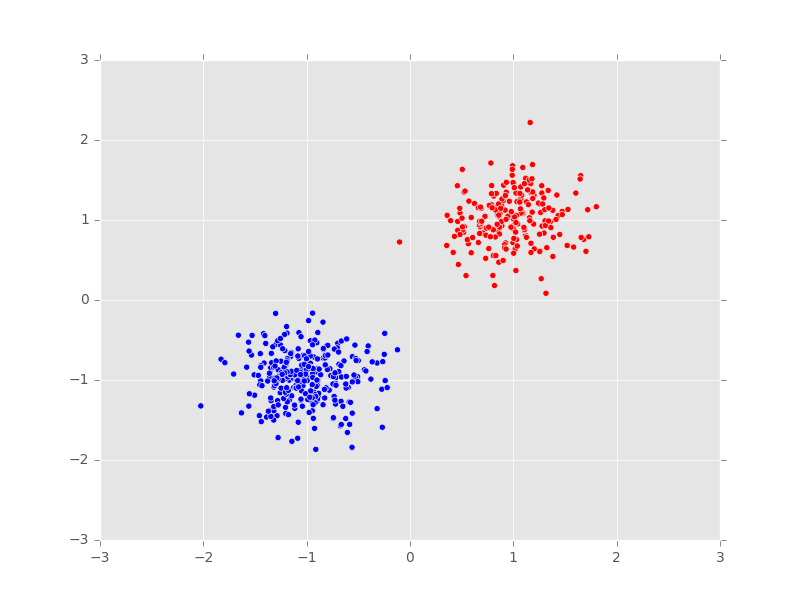
\includegraphics[width=700px]{/images/unsupervised-fig1.png}

\subsubsection{Remarks: The log-sum-exp trick}

For a collapsed mixture model, implementing the log density can be tricky.
In general, the log density is
\begin{align*}
  \log p(\pi) +
  \Big[ \sum_{k=1}^K \log p(\mathbf{\mu}_k) + \log
  p(\mathbf{\sigma}_k) \Big] +
  \sum_{n=1}^N \log p(\mathbf{x}_n \mid \pi, \mu, \sigma),
\end{align*}
where the likelihood is
\begin{align*}
  \sum_{n=1}^N \log p(\mathbf{x}_n \mid \pi, \mu, \sigma)
  &=
  \sum_{n=1}^N \log \sum_{k=1}^K \pi_k \, \text{Normal}(\mathbf{x}_n \mid
  \mu_k, \sigma_k).
\end{align*}
To prevent numerical instability, we'd like to work on the log-scale,
\begin{align*}
  \sum_{n=1}^N \log p(\mathbf{x}_n \mid \pi, \mu, \sigma)
  &=
  \sum_{n=1}^N \log \sum_{k=1}^K \exp\Big(
  \log \pi_k + \log \text{Normal}(\mathbf{x}_n \mid \mu_k, \sigma_k)\Big).
\end{align*}
This expression involves a log sum exp operation, which is
numerically unstable as exponentiation will often lead to one value
dominating the rest. Therefore we use the log-sum-exp trick.
It is based on the identity
\begin{align*}
  \mathbf{x}_{\mathrm{max}}
  &=
  \arg\max \mathbf{x},
  \\
  \log \sum_i \exp(\mathbf{x}_i)
  &=
  \log \Big(\exp(\mathbf{x}_{\mathrm{max}}) \sum_i \exp(\mathbf{x}_i -
  \mathbf{x}_{\mathrm{max}})\Big)
  \\
  &=
  \mathbf{x}_{\mathrm{max}} + \log \sum_i \exp(\mathbf{x}_i -
  \mathbf{x}_{\mathrm{max}}).
\end{align*}
Subtracting the maximum value before taking the log-sum-exp leads to
more numerically stable output. The \texttt{Mixture} random variable
implements this trick for calculating the log-density.

\subsubsection{References}\label{references}
